\documentclass{article}

\usepackage{xcolor}
\usepackage{inconsolata}
\usepackage[T1]{fontenc}
\usepackage{pgffor}
\usepackage{graphicx}
\usepackage{fancyhdr}
\usepackage{hyperref}
\usepackage{tcolorbox}
\usepackage[margin=1.2in]{geometry}
\usepackage{biblatex}
\addbibresource{refs.bib}

\hypersetup{
  colorlinks=true,
  linkcolor=blue,
  filecolor=magenta,
  urlcolor=blue,
}

\renewcommand*\familydefault{\ttdefault} %% Only if the base font of the document is to be typewriter style

\newcommand{\topic}[1]{\tcbox[on line,arc=4pt,colframe=white,boxrule=0pt,boxsep=0pt,left=4pt,right=4pt,top=3pt,bottom=2pt,colback=gray!30]{#1}}

% Define a custom command for colored boxes around words
\newcommand{\topics}[1]{%
  \linebreak
  \linebreak
  \foreach \word in {#1} {%
    \topic{\word}%
  }%
  \linebreak
}


\title{Exposé für eine Bachelorarbeit}
\author{Max Richter}

\begin{document}

\pagestyle{fancy}
\fancyhead{} % clear all header fields
\fancyhead[RO,LE]{\textbf{WebAssembly-basierten Visualen Programmiersprache}}
\fancyfoot{} % clear all footer fields
\fancyfoot[LE,RO]{\thepage}
\fancyfoot[LO,CE]{\href{https://github.com/jim-fx/bachelor}{github.com/jim-fx/bachelor}}
\fancyfoot[CO,RE]{Max Richter}

\raggedright

\maketitle
\pagebreak

{\LARGE Entwicklung einer Performanten WebAssembly-basierten Visualen Programmiersprache}
  
\section{Problemstellung}
In dieser Bachelorarbeit werde ich versuchen eine node-basierte visuelle Programmiersprache zu entwickeln, mit der Besonderheit das die einzelnen Nodes WebAssembly Module sind.
\begin{figure}[h]
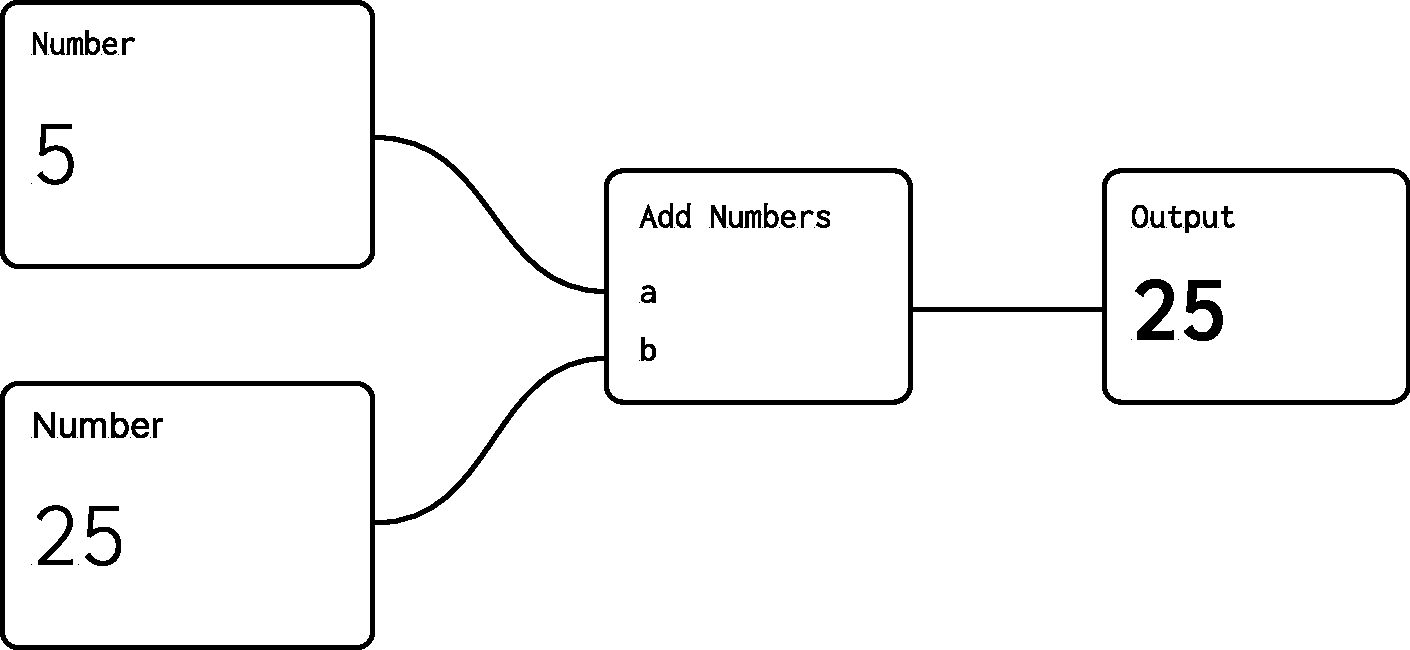
\includegraphics[width=\textwidth]{ideas/nodes.pdf}
\caption{Illustration eines Node-Systems}
\end{figure}
\linebreak
\linebreak
WebAssembly bietet sich hier gut an, da es plattformunabhängig, isoliert und performant ist \cite{Haas2017}. Gerade die Isolation der einzelnen Module ist spannend, da sie es möglich macht Nodes von unterschiedlichen Quellen zu laden, und trotzdem die Sicherheit des Hostsystems zu gewährleisten.
\linebreak
\linebreak
Dies wiederum würde es erlauben ein generelles Framework bereitzustellen bei denen Node-basierte UI's für unterschiedliche Usecases und dank der cross-plattform Eigenschaften von WebAssembly auch für unterschiedliche Plattformen erstellt werden können.

\section{Abgeleitete Forschungsfrage}
Diese Arbeit untersucht, ob eine node-basierte visuelle Programmiersprache, bei der die Nodes WebAssembly Module sind, implementiert werden kann und ob diese performant genug ist um in einem UI verwendet zu werden.

\section{Vorgehen}
\subsection{Literatur Recherche}
Als Erstes werde ich eine allgemeine Literaturrecherche zu den Themen \topic{WebAssembly}, \topic{visuelle Programmiersprachen} und im speziellen \topic{node-basierte visuelle Programmiersprachen} durchführen.

\subsection{Recherche von bestehenden Lösungen}
Node-basierte visuelle Programmiersprachen sind nichts Neues und es gibt viele bestehende Lösungen. Ich werde mir einige davon anschauen und analysieren.

\subsection{Implementierung}
Der Großteil der Arbeit wird in der Implementierung liegen. Hierbei sehe ich im Moment zwei Bereiche, die besonders interessant sind. Zum einen die Performance, da die Kommunikation zwischen einzelnen Nodes höchstwahrscheinlich über das Hostsystem laufen muss. Zweitens muss man eine Möglichkeit finden wie die einzelnen Nodes angeben welche Argumente sie erwarten. 
\linebreak
\linebreak
Die Implementierung wird im Kontext einer \href{https://plant.max-richter.dev}{3D-Anwendung} stattfinden, da ich in diesem Bereich viel Erfahrung habe. Außerdem werden in dieser speziellen Anwendung große Datenmengen zwischen den Nodes hin- und hertransportiert, was die Performance-Problematik gut verdeutlichen sollte.

\subsection{Evaluation}
Im letzten Schritt werde ich die Implementierung auf ihre Performance analysieren. Der Fokus hierbei wird auf der vom User wahrgenommenen Latenz liegen, da dies ein wichtiger Faktor für eine gute User-Experience ist. \cite{6876022}

\section{Formales}
Geplantes Startdatum: 10.01.2024
\linebreak
Sperrvermerk geplant: nein
\linebreak
Begründung: n.z.

\section{Externer Kooperationspartner}
n.z.

\printbibliography

\end{document}
